\documentclass[a4paper,11pt]{jsarticle}

% 数式
\usepackage{amsmath,amsfonts}
\usepackage{amsthm}
\usepackage{bm}
\usepackage{mathtools}
\usepackage{amssymb}

% 表
\usepackage[utf8]{inputenc}
\usepackage{diagbox} % 斜線付きセルを作成するために必要
\usepackage{booktabs} % 表の罫線を美しくするために必要
\usepackage{hhline} % 水平罫線を制御するために必要

% 画像
\usepackage[dvipdfmx]{graphicx}
\usepackage{ascmac}
\usepackage{physics}
\usepackage{float} % 追加

% 図
\usepackage[dvipdfmx]{graphicx}
\usepackage{tikz} %図を描く
\usetikzlibrary{positioning, intersections, calc, arrows.meta,math} %tikzのlibrary

% ハイパーリンク
\usepackage[dvipdfm,
  colorlinks=false,
  bookmarks=true,
  bookmarksnumbered=false,
  pdfborder={0 0 0},
  bookmarkstype=toc]{hyperref}

% 式番号を章ごとにリセット
\numberwithin{equation}{section}

\begin{document}

\title{B4ゼミ\#3}
\author{大上由人}
\date{\today}
\maketitle

\setcounter{section}{2}
\section{確率熱力学}
\subsection{Shanonエントロピー}
\subsubsection{Stochastic エントロピー}
\begin{itembox}[l]{\textbf{Def.Stochastic エントロピー}}
    M個の事象$\{x_1, x_2, \cdots, x_M\}$があるとき、事象$x_i$が起こる確率を$p_i$とする。このとき、事象$x_i$の確率的エントロピーは、
    \begin{align}
        s(x_i) = -\ln p_i
    \end{align}
    と定義される。
\end{itembox}
この量は、surprisalとも呼ばれ、ある事象がどれほど"驚くべき事象か"を表している。
例えば、$p_i = 1$のとき、$s(x_i) = 0$であるが、これは、事象$x_i$が起こることが確定しているので、"驚くべき事象"ではないことがわかる。
逆に、非常に確率が小さい事象$x_i$が起こるとき、$s(x_i)$は非常に大きな値をとる。これは、事象$x_i$が起こることは非常に驚くべき事象であることを表している。

Stochasticエントロピーは、以下の要素を満たす。
\begin{itemize}
    \item 確率分布$p_i$について連続関数である。
    \item 独立な分布$(p,p')$に対して、$s(p_p') = s(p) + s(p')$が成立する。
\end{itemize}
実は、この2つの条件を満たす関数は、$s(p) = -\ln p + C$の形のみであることが示される。

\begin{itembox}[l]{\textbf{Thm.}}
    $f(p)$が、以下の性質を持つとき、その関数形は定数項を除いて、$-\ln p$の形に一意に決まる。
    \begin{itemize}
        \item $f(p)$は、確率分布$p$に対して連続関数である。
        \item $f(p)$は、独立な分布$(p,p')$に対して、$f(p_p') = f(p) + f(p')$が成立する。
    \end{itemize}
\end{itembox}
\textbf{Prf.}\\
\indent
TODO後で書く。\qed\\

\subsubsection{Shanonエントロピー}
Stochasticエントロピーの平均として、Shanonエントロピーが定義される。

\begin{itembox}[l]{\textbf{Def.Shanonエントロピー}}
    $M$個の事象$\{x_1, x_2, \cdots, x_M\}$があるとき、事象$x_i$が起こる確率を$p_i$とする。このとき、確率変数$x$のShanonエントロピーは、
    \begin{align}
        H(x) = -\sum_{j} p_j \ln p_j
    \end{align}
    と定義される。
\end{itembox}
エントロピーは、事象の不確定性を表す量であるといえる。例えば、二項分布のエントロピーをグラフにすると、以下のようになる。
\begin{figure}[H]
    \begin{center}
    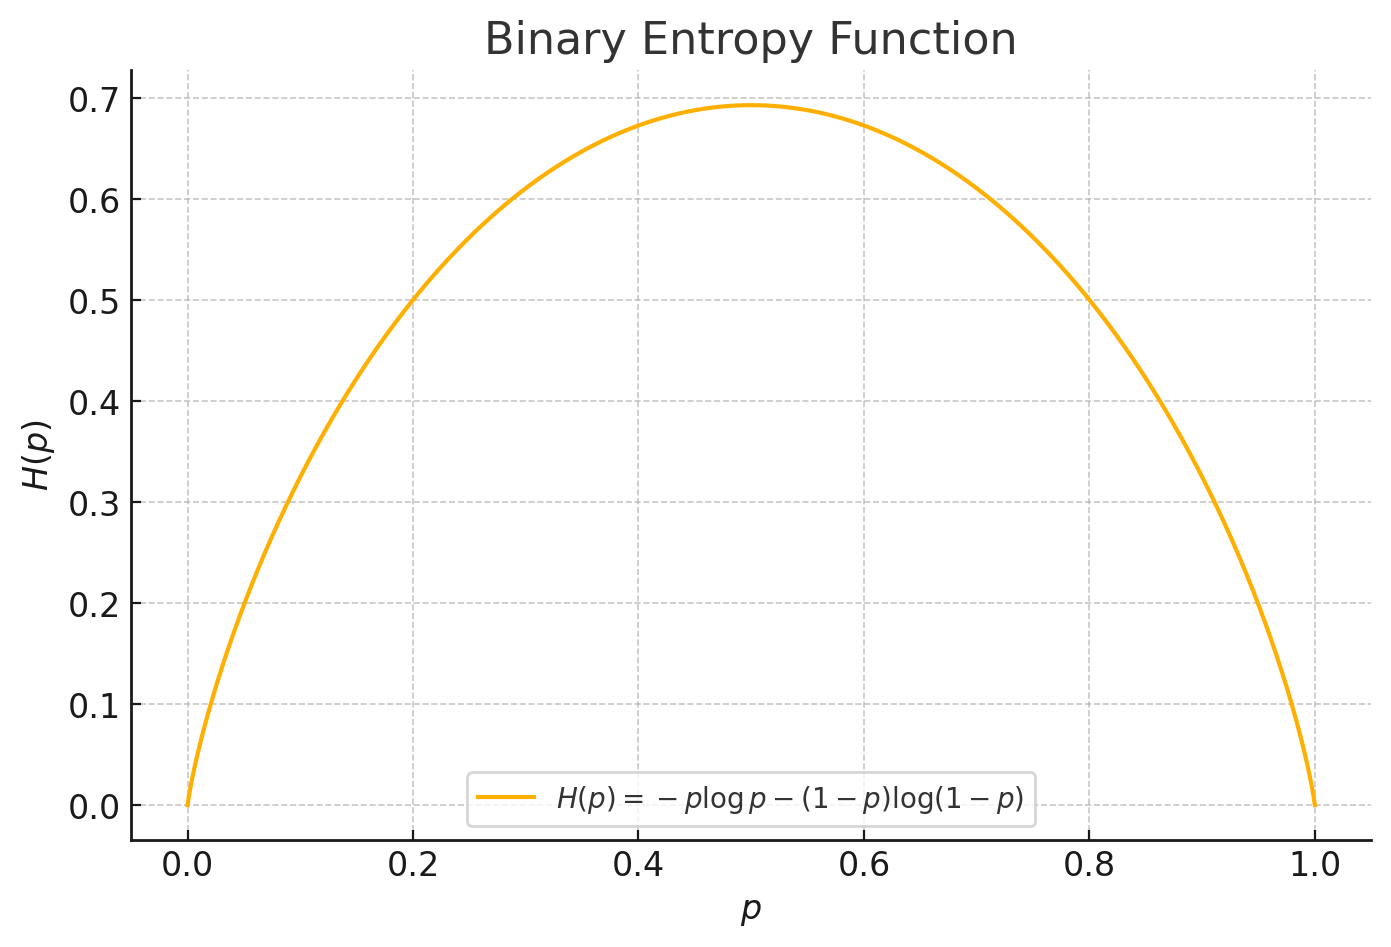
\includegraphics[width=100mm]{entropy.png}
    \end{center}
    \caption{二項分布のエントロピー}
    \label{fig:entropy}
\end{figure}
\indent
このとき、$p=\frac{1}{2}$のとき、エントロピーは最大値をとる。例えば、これをコイン投げに例えると、$p=\frac{1}{2}$のとき、表と裏が均等に出るので、コインを投げる前に、表が出るか裏が出るかは全くわからない。
しかし、$p\neq \frac{1}{2}$のとき、コインの出方が偏っているということになり、ある程度どちらが出るか予測できる。とくに、$p=0$または$p=1$のとき、エントロピーは0となるが、これは、事象の不確実性が0であることを表している。

条件付き確率についても、Shanonエントロピーは定義できる。
\begin{itembox}[l]{\textbf{Def.条件付きShanonエントロピー}}
    事象$y$のもとでの事象$x$のShanonエントロピーは、
    \begin{align}
        H(x|y) &= -\sum_{i,j}P(x_i,y_j) \ln P(x_i|y_j)\\
        &= -\sum_{j}P(y_j) \sum_{i}P(x_i|y_j) \ln P(x_i|y_j)
    \end{align}
    と定義される。
    ただし、$P(x_i,y_j)$は、事象$x_i$と$y_j$の同時分布である。
\end{itembox}
特徴をつかむために、コイントスの例を再び考えてみる。
TODO後で書く。\\

条件付き確率は、条件が付いている分、事象の不確実性が落ちているはずである。実際、以下が成り立つことが知られている。
\begin{itembox}[l]{\textbf{Thm.条件付けによるShanonエントロピーの単調性}}
    任意の確率変数$(x,y)$に対して、以下が成り立つ。 
    \begin{align}
        H(x|y) \leq H(x)
    \end{align}
\end{itembox}
この証明は、5章で行う。\footnote{KLダイバージェンスの正値性より従う。}\\

\subsection{熱の定義}
\subsubsection{平衡状態の時間反転対称性}


\end{document}